% flashcards-title: Forty-six marked between forty and fifty
% flashcards-desc: A number line runs from forty through fifty. Forty-six is marked, with comparison guides toward forty and fifty and forty-five labeled halfway.
\documentclass[dvisvgm,tikz,border=8pt]{standalone}
\usetikzlibrary{arrows.meta,patterns}

\definecolor{qraNavy}{HTML}{17324D}
\definecolor{qraBlue}{HTML}{2B6CB0}
\definecolor{qraGold}{HTML}{B7791F}
\definecolor{qraPale}{HTML}{EAF2F8}
\definecolor{qraGray}{HTML}{5C6773}

\tikzset{
  qra axis/.style={draw=qraNavy, line width=1.2pt},
  qra tick/.style={draw=qraNavy, line width=1pt},
  qra guide/.style={draw=qraGray, densely dashed, line width=0.8pt},
  qra counter/.style={circle, draw=qraNavy, fill=qraPale, line width=0.9pt, minimum size=7mm, inner sep=0pt},
  qra label/.style={font=\sffamily\bfseries, text=qraNavy},
  qra small label/.style={font=\sffamily, text=qraNavy},
}

\begin{document}
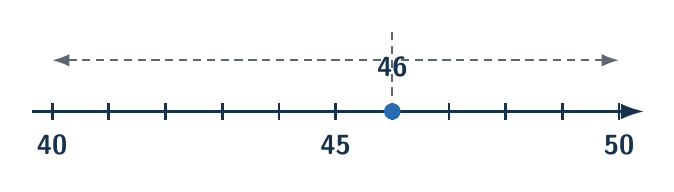
\begin{tikzpicture}[x=0.72cm,y=1cm]
  \draw[qra axis, -{Latex[length=3mm,width=2mm]}] (-0.35,0) -- (10.45,0);
  \foreach \x in {0,...,10} {
    \draw[qra tick] (\x,-0.11) -- (\x,0.11);
  }
  \node[qra label, below=5pt] at (0,0) {40};
  \node[qra label, below=5pt] at (5,0) {45};
  \node[qra label, below=5pt] at (10,0) {50};
  \draw[qra guide] (6,0.2) -- (6,1.05);
  \fill[qraBlue] (6,0) circle (3pt);
  \node[qra label, above=9pt] at (6,0) {46};
  \draw[qra guide, {Latex[length=2.2mm,width=1.6mm]}-] (0,0.65) -- (5.85,0.65);
  \draw[qra guide, -{Latex[length=2.2mm,width=1.6mm]}] (6.15,0.65) -- (10,0.65);
\end{tikzpicture}
\end{document}
